\subsection{Vektorräume}

\paragraph{Begriff:}
\begin{enumerate}
\item Gegeben seien ein Körper $(K,+,\cdot)$, dessen Elemente \emph{Skalare} heißen (meist $(\mathbb{R}, + ,\cdot)$) und eine ABELsche Gruppe $(V,\oplus)$ ($V$... Menge, Elemente heißen Vektoren, $\oplus$... Vektoraddition).
\item Es gibt eine Abbildung $\odot$ von $K\times V$ in $V$ die jedem $x \in V$ und jedem $\lambda \in K$ ein Element $\lambda \odot x$ in $V$ mit folgenden Eigenschaften zuordnet.
\begin{itemize}
\item Distributivgesetze: \\
$(\lambda + \mu)\odot x = (\lambda \odot x) \oplus (\mu \odot x)$\\
$\lambda\odot(x\oplus y)=(\lambda \odot x) \oplus (\lambda \odot y)$
\item Assoziativgesetz:\\
$(\lambda \cdot \mu ) \odot x = \lambda \odot (\mu \odot x)$
\item Neutrales Element:\\
$1 \odot x = x $
\end{itemize}
(für alle $\lambda, \mu \in K$ und $x,y\in V$)
\end{enumerate}
Eine Menge $V$ mit den in 1.) und 2.) aufgeführten Operationen $\oplus$ und $\odot$ heißt \emph{Vektorraum} (VR) \emph{über $K$}.\\
Bemerkung: Schreibweise meist $+$ anstelle von $\oplus$ und $\cdot$ anstelle von $odot$ (ergibt sich aus Zusammenhang der Elemente).
\subparagraph{Bsp. 1:} \parskp
Skalarbereich $\mathbb{R}$.\\
Vektoren: Größen, die durch eine Zahlenangabe (Länge) und eine Richtung charakterisiert sind (z.B. Kräfte, Geschwindigkeiten, Translatimen).\\
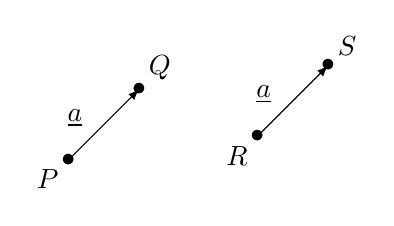
\begin{tikzpicture}[scale=0.3]
\draw[-latex] (0,0) -- (3,3);
\draw (0,0) node{$\bullet$};
\draw (0,0) node[below left] {$P$};
\draw (1,1) node[above left] {$\underline{a}$};
\draw (3,3) node[above right] {$Q$};
\draw (3,3) node{$\bullet$};

\draw[-latex] (8,1) -- (11,4);
\draw (8,1) node{$\bullet$};
\draw (8,1) node[below left] {$R$};
\draw (9,2) node[above left] {$\underline{a}$};
\draw (11,4) node[above right] {$S$};
\draw (11,4) node{$\bullet$};
\end{tikzpicture}\\
Pfeile als Repräsentanten eines Vektors $\underline{a}$.\\
Bezeichnung: $\underline{a}=\overrightarrow{a}=\overrightarrow{PQ}=\overrightarrow{RS}$
\paragraph{Ortskurven:} Angeheftet in gemeinsamen Anfangspunkt $O$ (Ursprung).
\begin{itemize}
\item Vektoraddition: $\underline{a}+\underline{b}$ ABB 110
\item Multiplikation mit Skalar: $\lambda \cdot \underline{a}$:\\
$\lambda > 0$ ABB 111\\
$\lambda < 0$ ABB 112\\
Länge von $\lambda \cdot \underline{a}$ ist das $|\lambda|$-fache der Länge von $\underline{a}$.
\item Subtraktion: $\underline{a}-\underline{b}=\underline{a}+(-\underline{b})=\underline{a}+((-1)\cdot \underline{b})$ ABB 113
\item Nullvektor: $\underline{0}$ (Länge 0, keine Richtung)
\end{itemize}
\subparagraph{Bsp. 2:} \parskp
$K = \mathbb{R}, V = \left\lbrace \begin{pmatrix}
x_1\\ x_2 \\ ... \\ x_n
\end{pmatrix}, x_1, x_2, ..., x_n \in \mathbb{R}\right\rbrace$\\
Vektoraddition: $\begin{pmatrix}
x_1\\ x_2 \\ ... \\ x_n
\end{pmatrix} + \begin{pmatrix}
y_1\\ y_2 \\ ... \\ y_n
\end{pmatrix}=\begin{pmatrix}
x_1+y_1\\ x_2+y_2 \\ ... \\ x_n+y_3
\end{pmatrix}$\\
Multiplikation mit Skalar: $\lambda \cdot \begin{pmatrix}
x_1\\ x_2 \\ ... \\ x_n
\end{pmatrix} = \begin{pmatrix}
\lambda \cdot x_1\\ \lambda \cdot x_2 \\ ... \\  \lambda \cdot x_n
\end{pmatrix}$\medskip\\
$\curvearrowright$ $V$ Vektorraum über $\mathbb{R}$, Bezeichnung: $\mathbb{R}^n$, Nullvektor $\begin{pmatrix}
0\\ 0 \\ ... \\ 0
\end{pmatrix}$
\paragraph{Def. 1:} \parskp
Die Vektoren $\underline{a}_1, ..., \underline{a}_n$ heißen \emph{linear unabhängig}, wenn die Gleichung $\boxed{x_1\underline{a}_1+...+x_n\underline{a}_n=\underline{0}}$ nur die triviale Lösung $x_1=x_2 = .... =x_n = 0$ besitzt.
\subparagraph{Diskussion:}
\begin{enumerate}
\item $x_1\underline{a}_1+...+x_n\underline{a}_n$ heißt \emph{Linearkombination} (LK) der Vektoren $\underline{a}_1, ..., \underline{a}_n$.
\item Falls es eine darstellung der Gestalt wie in Def. 1 gibt, in der nicht alle $x_i$ gleich 0 sind, so heißen $\underline{a}_1, ..., \underline{a}_n$ \emph{linear unabhängig}.\\
In diesem Falle lässt sich (wenigstens) einer der Vektoren als LK der anderen darstellen.
\end{enumerate}

\paragraph{Def. 2:} \parskp
Es sei $V_1 \subseteq V$ eine nichtleere Teilmenge von $V$. Wir bezeichnen mit $L(V_1)$ die Menge \emph{aller} LK von jeweils endlich vielen Vektoren aus $V_1$. $L(V_1)$ ist die sogenante \emph{lineare Hülle} von $V_1$.
\subparagraph{Bemerkung:} \parskp
$L(V_1)$ ist selbst ein Vektorraum, nämlich der von $V_1$ aufgespannte Teilraum von $V$ (kleinster VR, welcher $V_1$ enthält).

\paragraph{Def. 3:}
\begin{itemize}
\item Ein Vektorraum $V$ heißt \emph{n-dimensional}, wenn es $n$ linear unabhängige Vektoren $\underline{a}_1, ..., \underline{a}_n$ gibt, die den gesamten Raum aufspannen ($L(\{\underline{a}_1, ..., \underline{a}_n\})=L(\underline{a}_1, ..., \underline{a}_n)=V$).
\item Die Menge der Vektoren $\underline{a}_1, ..., \underline{a}_n$ nennt man in diesem Falle eine Basis von $V$.
\end{itemize}
\subparagraph{Diskussion:}\parskp
In einem Vektorraum gibt es unterschiedliche Basen, jedoch ist die Anzahl der Vektoren, die eine Basis bilden, stets gleich (Dimension des VR).
\paragraph{Satz 1:}\parskp
Es sei $\underline{a}_1, ..., \underline{a}_n$ eine Basis des VRs $V$. Dann gibt es für \emph{jedes} $\underline{x}\in V$ eine \emph{eindeutige} Darstellung der Gestalt $\underline{x}=x_1\underline{a}_1, ..., x_n\underline{a}_n$.
\subparagraph{Bemerkung:}
\begin{itemize}
\item Die Koeffizienten $x_1,...x_n$ heißen \emph{Koordinaten} von $\underline{x}$ bezüglich der Basis $\underline{a}_1, ..., \underline{a}_n$.
\item Die Summanden $x_1\underline{a}_1, ..., x_n\underline{a}_n$ heißen \emph{Komponenten} von $\underline{x}$ bezüglich der Basis $\underline{a}_1, ..., \underline{a}_n$.
\end{itemize}
\subparagraph{Bsp. 3:} \parskp
Die Vektoren $\underline{e}_1=\begin{pmatrix}
1\\0\\...\\0
\end{pmatrix}, \underline{e}_2=\begin{pmatrix}
0\\1\\...\\0
\end{pmatrix}, ..., \underline{e}_N=\begin{pmatrix}
0\\0\\...\\1
\end{pmatrix}$des Raumes $\mathbb{R}^n$ bilden offensichtlich eine Basis von $\mathbb{R}^n$.\\
$\curvearrowright \underline{e}_1, ..., \underline{e}_n$ sind linear unabhängig. Ferner gilt für beliebiges $\underline{x}=\begin{pmatrix}
x_1 \\ ...\\ x_n
\end{pmatrix}\in \mathbb{R}^n$. $\underline{x}=x_1\cdot \underline{e}_1+...+x_n \cdot \underline{e}_n$.
\subparagraph{Bsp. 4:} \parskp
Zwei Vektoren $\underline{a}_1 \not = \underline{0}$ und $\underline{a}_2 \not = \underline{0}$ in einer Ebene bilden genau dann eine Basis, wenn sie nicht parallel sind.

\subsection{Matrizen}

\paragraph{Def. 4:} \parskp
Ein aus $m\cdot n$ Zahlen $a_{ij}\in \mathbb{R}$, welche in $m$ Zeilen und $n$ Spalten angeordnet sind, bestehendes Schema heißt \emph{Matrix vom Typ $(m,n)$}.\\
$\underline{A}=\begin{pmatrix}
a_{11} & a_{12} & a_{13}& ... &a_{1n}\\
a_{21} & a_{22} & a_{23}& ... &a_{2n}\\
... & ... & ... &... & ...\\
a_{m1} & a_{m2} & a_{m3} &...& a_{mn}\\
\end{pmatrix}=(a_{ij})_{\substack{i=1,...,m \text{ (Zeilenindex)} \\ j=1,...,n \text{ (Spaltenindex)}}}
$

\paragraph{Def. 5} Rechenoperationen
\begin{enumerate}
\item $\underline{A}=(a_{ij}), \underline{B}=(b_{ij})$ seien vom gleichen Typ $(m,n)$.\\
$\boxed{\underline{A}+\underline{B}:= (a_{ij}+b_{ij})}$ \emph{Addition von Matrizen}
\item Sei $\lambda \in \mathbb{R}$ und $\underline{A}=(a_{ij})$ vom Typ $(m,n)$.\\
$\boxed{\lambda\cdot \underline{A}=(\lambda\cdot a_{ij})}$ \emph{Multiplikation einer Matrix mit einem Skalar}
\item $\underline{A}=(a_{ij}$ sei vom Typ $(m,n)$\\
$\underline{B}=(b_{ij})$ sei vom Typ $(n,p)$\\
$\underline{A}$ und $\underline{B}$ heißen in dieser Reihenfolge \emph{verkettet} (Spaltenzahl von $\underline{A}$ = Zeilenzahl von $\underline{B}$).\\
$\boxed{\underline{A}\cdot \underline{B}= \left( \sum_{j=1}^{n} a_{ij}\cdot b_{jk}\right)_{\substack{i=1,...,m \\ k= 1,...,p}}}$ \emph{Matrizenmultiplikation}\\
Das Produkt ist also vom Typ $(m,p)$.
\end{enumerate}
\subparagraph{Diskussion:} \parskp
Zweckmäßig FALK-Schema zur Matrizenmultiplikation (vgl. folgendes Bsp. 5).

\paragraph{Def. 6} \parskp
Die  aus der $(m,n)$-Matrix $\underline{A}$ durch Vertauschung von Zeilen und Spalten entstehende $(n,m)$-Matrix heißt \emph{Transformierte} von $\underline{A}$. Bezeichnung: $\underline{A}^T$.

\subparagraph{Bsp. 5:} \parskp
$\underline{A}=\begin{pmatrix}
5 & -3\\
1 & 4\\
\end{pmatrix}, \underline{B}=\begin{pmatrix}
3 & 6 & 4\\
-2 & 0 & 1\\
\end{pmatrix}, \underline{C}=\begin{pmatrix}
-1 & 5\\
0 & 3\\
\end{pmatrix}$
\begin{enumerate}[label=\alph*.)]
\item $\underline{A}+\underline{B}$ existiert nicht (unterschiedliche Typen).
\item $\underline{A}+\underline{C}=\begin{pmatrix}
4 & 2\\
1 & 7\\
\end{pmatrix}$
\item $2\cdot \underline{A}=\begin{pmatrix}
10 & -6\\
2 & 8\\
\end{pmatrix}$
\item $\underline{B}^T=\begin{pmatrix}
3 & -2\\
6 & 0\\
4 & 1\\
\end{pmatrix}$
\item $\underline{B}\cdot \underline{A}$ existiert nicht ($(2,3)$ und $(2,2)$ nicht verkettet)
\item $\underline{A}\cdot \underline{B}=\begin{pmatrix}
21 & 30 & 17\\
-5 & 6 & 8\\
\end{pmatrix}$\\
(mit FALK-Schema:)
\begin{tabular}{c c | c c c}
 & & 3 & 6& 4\\
 & & -2 & 0 & 1\\
\hline
5 & -3 & 21 & 30 & 17\\
1 & 4 &  -5& 6 & 8\\
\end{tabular}\\
Bemerkung: Die Matrizenmultiplikation ist nicht kommutativ!
\end{enumerate}
\subparagraph{Diskussion:} (ausgewählte Rechenregeln)
\begin{enumerate}
\item Die Menge der Matrizen vom gleichen Typ bilden mit den Operationen Addition und Multiplikation mit einem Skalar einen Vektorraum.\\
Bsp:  $V=\{\text{Matrizen vom Typ }(2,2)\}$\\
Basis: $\begin{pmatrix}
1& 0\\
0 &0 \\
\end{pmatrix},\begin{pmatrix}
0& 1\\
0 &0 \\
\end{pmatrix},\begin{pmatrix}
0& 0\\
1 &0 \\
\end{pmatrix},\begin{pmatrix}
0& 0\\
0 &1 \\
\end{pmatrix}$
\item Falls die entsprechenden Typvoraussetzungen erfüllt sind, gelten: 
\begin{itemize}
\item $(\underline{A}\cdot \underline{B})\cdot \underline{C}=\underline{A}\cdot (\underline{B}\cdot \underline{C})$ (Assoziativgesetz)
\item $(\underline{A}\cdot \underline{B})+ \underline{C}=\underline{A}\cdot \underline{B}+ \underline{A}\cdot \underline{C}$\\
$(\underline{A}+ \underline{B})\cdot \underline{C}=\underline{A}\cdot \underline{C}+ \underline{B}\cdot \underline{C}$ (Distributivgesetze)
\item $(\lambda \cdot \underline{A})\cdot \underline{B}=\lambda \cdot (\underline{A}\cdot \underline{B})=\underline{A}\cdot (\lambda\cdot \underline{B})$
\item $(\lambda \cdot \underline{A})^T=\lambda \cdot \underline{A}^T \qquad \left(\underline{A}^T\right)^T=\underline{A}$
\item $(\underline{A}+\underline{B})^T=\underline{A}^T+\underline{B}^T
 \qquad \boxed{\left(\underline{A}\cdot \underline{B}\right)^T=\underline{B}\cdot \underline{A}^T}$
\end{itemize}
\item Achtung: Im Allgemeinen gilt $\underline{A} \cdot \underline{B} \not = \underline{B} \cdot \underline{A}$!
\item FALK-Schema bei fortgesetzter Multiplikation $\underline{A}\cdot \underline{B}\underline{C}$\\
\begin{tabular}{c | c | c}
 & $\underline{B}$ & $\underline{C}$\\
 \hline
$\underline{A}$ & $\underline{A}\cdot\underline{B}$ & $(\underline{A}\cdot\underline{B})\cdot \underline{C}$
\end{tabular} oder 
\begin{tabular}{c | c}
 & $\underline{C}$\\
\hline
$\underline{B}$ & $\underline{B}\cdot \underline{C}$\\
$\underline{A}$ & $\underline{A}\cdot (\underline{B}\cdot \underline{C})$\\
\end{tabular} (2 Varianten, gemäß Assoziativgesetz)
\end{enumerate}
\paragraph{Spezielle Matrizen}
\begin{enumerate}
\item \emph{Quadratische Matrizen}: Typ $(n,n)$\\
Eine quadratische Matrix $\underline{A}$ heißt
\begin{enumerate}
\item \emph{symmetrisch}, wenn $\underline{A}^T=\underline{A}$ gilt.
\item obere \emph{Dreiecksmatrix}, wenn $a_{ij}=0$ für $i>j$.\\
untere \emph{Dreiecksmatrix}, wenn $a_{ij}=0$ für $i<j$.
\item \emph{Diagonalmatrix}, wenn $a_ij=$ für $i\not = j$.
\item \emph{Einheitsmatrix} $\underline{E}$, wenn $a_{ij}=\begin{cases}
1 \quad \text{für }i=j\\
0 \quad \text{für } i \not = j\\
\end{cases}$ (spezielle Diagonalmatrix). \\
$\underline{E}=\begin{pmatrix}
1 & 0 & ... &0 \\
0 & 1 & ... &0 \\
... &... & ... & ...\\
0 & 0 & ... & 1 \\
\end{pmatrix}$
\end{enumerate}
\item \emph{Nullmatrix} $\underline{0}$ (sämtliche Elemente $0$, nicht notwendig quadratisch).
\item Matrizen vom Typ $(n,1)$ ($n$ Zeilen, eine Spalte) heißen (Spalten-)Vektoren.\\
$\underline{a}=\begin{pmatrix}
a_1\\
a_2\\
...\\
a_n
\end{pmatrix} \in \mathbb{R}^n$ (vgl. \ref{ 5.1})\\
Es ist $\underline{a}^T=(a_1| a _2 | ... | a_n)=\begin{pmatrix}
a_1 & a_2 & ... & a_n\\
\end{pmatrix}$ vom Typ $(1,n)$ (Zeilenvektor).
\end{enumerate}
\subparagraph{Diskussion:}
\begin{enumerate}
\item Die quadratischen Matrizen vom Typ $(n,n)$ bilden mit den Operationen Addition und Multiplikation von Matrizen einen (nicht kommutativen) Ring.
\item Für quadratische Matrizen $\underline{A}$ sind Potenzen bildbar: \\
$\boxed{\underline{A}^0=\underline{E} \quad \underline{A}^n=\underbrace{\underline{A}\cdot\underline{A}\cdot ... \cdot\underline{A}}_{n-\text{Faktoren}}, n \in \mathbb{N}}$
\item Falls die entsprechenden Typvoraussetzungen erfüllt sind, gelten:\\
$\underline{A}\cdot \underline{E}=\underline{A}\\
\underline{E}\cdot \underline{A}=\underline{A}\\
\underline{0}\cdot \underline{A} = \underline{0}\\
\underline{A} \cdot \underline{0} = \underline{0}\\
\underline{A} + \underline{0} = \underline{A}\\
\underline{0} + \underline{A} = \underline{A}$\\
(analog $0$ und $1$ bei den reellen Zahlen)
\item Sei $\underline{A}$ vom Typ $(m,n)$, $x \in \mathbb{R}^n$, d.h. vom Typ $(n,1)$.\\ Dann ist $\boxed{\underline{y}= \underline{A} \cdot \underline{x}}$ vom Typ $(m,1)$.\\
Durch die Zuordnung $\underline{x}\longmapsto \underline{A}\cdot \underline{x} = \underline{y}$ wird eine \emph{lineare Abbildung} von $\mathbb{R}^n$ in $\mathbb{R}^m$ beschrieben (Fkt. $f$ heißt linear, wenn gilt $f(x+y)=f(x)+f(y)$ und $f(\alpha \cdot x)=\alpha \cdot f(x)$ für alle $\alpha \in \mathbb{R}, \; x,y \in Db(f)$ gilt).
\end{enumerate}

\subsection{Determinanten}
\paragraph{Def. 7:} \parskp
Jeder $n$-reihigen quadratischen Matrix ist eindeutig eine Zahl $det\;\underline{A}$, die sogenannte \emph{Determinante} von $\underline{A}$, wie folgt zugeordnet.\\
$n=1$: $det\left((a_{11})\right):=a_{11}$\\
$n\geq 2$: $det\left(\begin{pmatrix}
a_{11} & ... & a_{1n}\\
...	&	& ...\\
a_{n1} &...&a_{nn}
\end{pmatrix}
\right):= a_{11}A_{11}+a_{12}A_{12}+...+a_{1n}A_{1n}$.\\
Dabei ist $A_{ij}=(-1)^{i+j} det\; U_{ij}$ die \emph{Adjunkte} des Elements $a_{ij}$.\\
$U_{ij}$ ist die $(n-1)$-reihige \emph{(Unter-)Matrix}, die durch Streichen der $i$-ten Zeile und der $j$-ten Spalte von $\underline{A}$ ernsteht.\\
Bezeichnung: $det(\underline{A})=det\left(\begin{pmatrix}
... & ...\\
... & ...\\
\end{pmatrix}\right)=\begin{vmatrix}
a_{11} & ... & a_{1n}\\
...	&	& ...\\
a_{n1} &...&a_{nn}
\end{vmatrix}$
\subparagraph{Bsp. 6:}
\begin{enumerate}[label=\alph*.)]
\item $n=2$: \\
$\begin{vmatrix}
a_{11} &  a_{12}\\
a_{21} &a_{22}
\end{vmatrix}\\
=a_{11}A_{11}+a_{12}A_{12}=a_{11}\cdot (-1)^{1+1}\cdot a_{22}+a_{12}\cdot(-1)^{1+2}\cdot a_{21}\\
=\resultul{a_{11}\cdot a_{22}-a_{12}\cdot a_{21}}$
\item $n=3$: \\
$\begin{vmatrix}
a_{11} &  a_{12} & a_{13}\\
a_{21} &a_{22} & a_{23}\\
a_{31} & a_{32} & a_{33}
\end{vmatrix}\\
=a_{11}A_{11}+a_{12}A_{12}+a_{13}A_{13}\\
=a_{11} \begin{vmatrix}
a_{22} & a_{23}\\
a_{32} & a_{33}\\
\end{vmatrix}-a_{12}\begin{vmatrix}
a_{21} & a_{23}\\
a_{31} & a_{33}
\end{vmatrix}+a_{13} \begin{vmatrix}
a_{21} & a_{22}\\
a_{31} & a_{32}
\end{vmatrix}\\
=a_{11}a_{22}a_{33}+a_{12} a_{23}a_{31}+a_{13} a_{21} a_{32}-(a_{13} a_{22} a_{31}+a_{11}a_{23}a_{32}+a_{12}+a_{21}+a_{33})
$\medskip\\
(Alternativ auch: Regel von SARRUS [diese gilt NUR für 3-reihige Determinanten] $\Rightarrow$ (Summe der Produkte der Diagonalen nach rechts unten)-(Summe der Produkte der Diagonalen nach links unten))
\end{enumerate}
\paragraph{Satz 2:}
\begin{enumerate}[label=\alph*.)]
\item $det(\underline{A}\cdot \underline{B}) = det (\underline{A})\cdot det(\underline{B})$
\item $det(\underline{A})=det(\underline{A}^T)$
\end{enumerate}
Wegen Satz 2b gelten für alle folgenden, für die Zeilen formulierten Eigenschaften auch sinngemäß für die Spalten.
\paragraph{Satz 3:} (Eigenschaften der Determinante)
\begin{enumerate}[label=(E\arabic*)]
\item $\underline{B}$ gehe aus $\underline{A}$ durch Vertauschen zweier Zeilen hervor, dann gilt $det(\underline{B})=-det(\underline{A})$.
\item Es gilt $det(\underline{A})=0$ falls zwei Zeilen elementweise proportional sind bzw. falls alle Elemente einer Zeile gleich $0$ sind. 
\item Es gilt $\begin{vmatrix}
a_{11} & ... & a_{1n}\\
... &  & ...\\
\lambda a_{i1} & ... & \lambda a_{in}\\
... & & ...\\
a_{n1} & ... & a_{nn}
\end{vmatrix}=\lambda\begin{vmatrix}
a_{11} & ... & a_{1n}\\
... &  & ...\\
a_{i1} & ... & a_{in}\\
... & & ...\\
a_{n1} & ... & a_{nn}
\end{vmatrix}$ (steht ein Faktor in einer Zeile einer Determinante, so kann er auch vorgezogen werden).
\item Der Wert einer Determinante ändert sich nicht, wenn das $\lambda$-fache einer Zeile elementweise zu einer anderen Zeile addiert wird.
\item $det(\underline{A})=\sum_{j=1}^{n}a_{ij}A_{ij}$ (Entwicklung nach $i$-ter Zeile, $(i=1,...,n)$)\\
$det(\underline{A})=\sum_{i=1}^{n}a_{ij}A_{ij}$ (Entwicklung nach $j$-ten Spalte, $(j=1,...,n)$)\\
$\rightarrow$ \emph{Entwicklungssatz}
\end{enumerate}
\paragraph{Bsp. 7:} \parskp
$\begin{vmatrix}
1 & 1 & 3 & -1\\
-2 & 2& -5& -4\\
-1 & 1 & -4 & 2\\
6 & 2 &-1 & 0
\end{vmatrix}$\\
3. Spalte = Arbeitsspalte (bleibt unverändert)\\
Um in der untersten Spalte mehr Nullen zu erzeugen (mit Regel E4):\\
$S_{1,neu}:=S_1+6\cdot S_3\\
S_{2,neu}:=S_2+2\cdot S_3$\\
$\Rightarrow$\\
$=\begin{vmatrix}
19 & 7 & 3 & -1\\
-32 & -8& -5& -4\\
-26 & -7 & -4 & 2\\
0 & 0 &-1 & 0
\end{vmatrix}$\\
Nun kann mit der letzen Zeile relativ einfach die Determinante berchnet werden:\\
$=(-1)\cdot (-1)^{4+3}\cdot \begin{vmatrix}
19 & 7 &-1\\
-32 & -8 & -4\\
-26 & -7 & 2\\
\end{vmatrix}$\\
Auf gleiche Weise werden nun wieder in Zeilen Nullen erzeugt:\\
$Z_{2,neu}:=Z_2-4Z_1\\
Z_{3,neu}:=Z_3+2Z_1$\\
$\Rightarrow$\\
$=\begin{vmatrix}
19 & 7 & 1\\
-108 & -36 & 0\\
12 & 7 &0
\end{vmatrix}\\
=(-1)\cdot (-1)^{1+3}\begin{vmatrix}
-108 & -36\\
12 & 7
\end{vmatrix}\\
\overset{E3}{=}(-1)\cdot (-36) \cdot \begin{vmatrix}
3 & 1 \\
12 & 7
\end{vmatrix}=36 \cdot 9 = \resultul{324}$\\
Prinzip: Nullen erzeugen mit (E4), dann mit Entwicklungssatz lösen (E5).
\paragraph{Anwendungen}
\begin{enumerate}
\item Vekotorrechnung in $\mathbb{R}^3$ (vgl. später, Abschnitt 5.5 \ref{5.5})
\item Gegeben sei ein lineares Gleichungssytem ($n$ Gleichungen, $n$ Unbekannte)\\
Matrixform $\boxed{\underline{A}\cdot \underline{x}=\underline{b}}$ mit $\underline{A}=(a_{ij}), \underline{x}=\begin{pmatrix}
x_1\\
...\\
x_n
\end{pmatrix}, \underline{b}=\begin{pmatrix}
b_1\\
...\\
b_n
\end{pmatrix}$. Diese Matrixform besitzt genau dann eine eindeutige Lösung $\underline{x}$, wenn $det(\underline{A})\not = 0$. \\
In diesem Falle gilt $\boxed{x_j=\frac{det(\underline{B}_j)}{det(\underline{A})}}\; (j=1,...,n)$. Wobei $\underline{B}_j$ aus $\underline{A}$ hervorgeht, indem man die $j$-te Spalte durch $\underline{b}$ ersetzt (\emph{CRAMERsche Regel}, theoretische Bedeutung, praktisches Vorgehen zur Lösung der Matrixform vgl. folgenden Abschnitt).
\end{enumerate}

\subsection{Lineare Gleichungssysteme, Rang einer Matrix, Inverse}
\subsubsection{Das Austauschverfahren}
Gegeben sei System von $m$ linearen Funktionen mit den unabhängigen Veränderlichen $x_1,...,x_n$ und den abhängigen Veränderlichen $y_1,...,y_n$.
\begin{align*}
y_1&= a_{11}x_{1}+a_{12}x_{2}+...+a_{1n}x_{n}+a_{10}\\
y_2&= a_{21}x_{1}+a{22}x_{2}+...+a{2n}x_{n}+a_{20}\\
...\\
y_m&=a_{m1}x_{1}+a{m2}x_{2}+...+a{mn}x_{n}+a_{m0}
\end{align*}

\subparagraph{Bsp. 8:}\parskp
Betrieb, in Abteilungen, $n$ Produkte $P_1,...,P_n$:\\
$a_{ij}$... Kosten pro Einheit von $P_j$ die in Abteilung $i$ entstehen.\\
$a_{i0}$... Fixkosten in Abteilung $i$.\\
$x_{j}$... produzierte Mengen von $P_j$.\\
$y_{i}$... Gesamtkosten in Abteilung $i$.\medskip\\
Matrix-Schreibweise: $\underline{y}=\underline{A}\,\underline{x}+\underline{a}$ mit $\underline{A}=(a_{ij})_{\substack{i=1,...,m\\j=1,...,n}},\; \underline{a}=\begin{pmatrix}
a_{01}\\
...\\
a_{0m}
\end{pmatrix}$\\
Tabellenform:\\
\begin{tabular}{c | c c c c c}
& $x_1$ & $x_2$ & ... & $x_n$ & 1\\
\hline
$y_1$ & $a_{11}$ & $a_{12}$ & ... & $a_{1n}$ & $a_{10}$\\
$y_2$ & $a_{21}$ & $a_{22}$ & ... & $a_{2n}$ & $a_{20}$\\
... & ... & & & & \\
$y_m$ & $a_{m1}$ & $a_{m2}$ & ... & $a_{mn}$ & $a_{m0}$\\
\end{tabular} bzw. 
\begin{tabular}{c | c c}
& $x^T$ & $1$\\
\hline
$\underline{y}$ & $\underline{A}$ & $\underline{a}$\\
\end{tabular}\\
Aufgaben:
\begin{enumerate}
\item $\underline{x}$ vorgegeben, $\underline{y}$ ist zu berechnen (klar!).
\item $\underline{y}$ vorgegeben, $\underline{x}$ zu berechnen (nicht immer lösbar, falls lösbar, nicht immer eindeutig lösbar).
\end{enumerate}
Lösungsprinzip:\\
Man tausche so oft wie möglich $y_r$ gegen $x_s$ aus, Austauschschritt AS ($y_r\leftrightarrow x_s$) $\rightarrow$ \emph{Austauschverfahren}.\\
Austauschschritt $y_r\leftrightarrow x_s$ bedeutet:
\begin{enumerate}
\item $r$-te Zeile $y_r=...$ nach $x_s$ auflösen $x_s=...$.
\item in allen anderen Zeilen $x_s$ durch die rechte Seite vom obigen $x_s$ ersetzen.\\
$\curvearrowright$ neue Tabelle
\end{enumerate}
FOLIEN IM NETZ (Neumann)\\
Praktisches Vorgehen:
\begin{enumerate}
\item Pivotelement (Pivot) kennzeichnen $\circ$
\item Austauschregeln Austauschregel (AR) 1 bis AR 4 abarbeiten\\
Dabei für AR 4 unter der alten Tabelle die neue Pivotzeile (PZ) als Kellerzeile notieren.
\end{enumerate}
ABB51\\
$a_{ij}^{*}=a_{ij}+a_{is}\cdot a_{rj}^{*}$ (Rechteckregel)
\subparagraph{Bsp. 8} (Fortsetzung)\\
$y_1=2x_1+3x_2+x_3+50$ (Kosten in Abt. 1)\\
$y_2=x_1+2x_3+40$ (Kosten in Abt. 2)\\
\begin{tabular}{c | c c c c}
$T_1$ & $x_1$ & $x_2$ & $x_3$ & $1$\\
\hline
$y_1$ & 2 & 3 & \fbox{1} & 50\\
$y_2$ & 1 & 0 & 2 & 40\\
\hline
K & -2 & -3 & * & -50
\end{tabular} \quad
\begin{tabular}{c | c c c c}
$T_2$ & $x_1$ & $x_2$ & $y_1$ & $1$\\
\hline
$x_3$ & -2 & -3 & 1 & -50\\
$y_2$ & \fbox{-3} & -6 & 2 & -60\\
\hline
K & * & -2 & $\tfrac{2}{3}$ & -20
\end{tabular}\quad
\begin{tabular}{c | c c c c}
$T_3$ & $y_2$ & $x_2$ & $y_1$ & $1$\\
\hline
$x_3$ & $\tfrac{2}{3}$ & 1 & $-\tfrac{1}{3}$ & -10\\
$x_1$ & $-\tfrac{1}{3}$ & -2 & $\tfrac{2}{3}$ & -20\\
\hline
\\
\end{tabular}\\
d.h.:\\
$x_3=\frac{2}{3}y_2 + x_2 - \frac{1}{3}y_1 - 10$\\
$x_1=-\frac{1}{3} y_2 - 2x_2 + \frac{2}{3}y_1-20$\\
$\curvearrowright$ bei vorgegebenen Kosten $y_1, y_2$ ist die Lösung $\underline{x}=\begin{pmatrix}
x_1\\x_2\\x_3
\end{pmatrix}$ nicht eindeutig bestimmbar.\\
 z.B. $y_1=600,\; y_2=300$:\\
$x_2=t$ (\emph{frei wählbar})\\
$x_3=\frac{2}{3}\cdot 300 + t - \frac{1}{3}\cdot 600 -10 = t-10\\
x_1=-\frac{1}{3}\cdot 300 - 2t + \frac{2}{3}\cdot 600 -20=280-2t\\
\Rightarrow \underline{x}=\begin{pmatrix}
280-2t\\
t\\
t-10
\end{pmatrix}$\\
hier für $x_i\geq 0$: $10\leq t \leq 140$.
\bigskip\\
Varianten des Austauschverfahrens (AV)
\begin{enumerate}
\item AVZ … Austauschverfahren mit \emph{Zeilentilgung}, d.h. neue PZ in neuer Tabelle weglassen.
\item AVS … Austauschverfahren mit \emph{Spaltentilgung}, d.h. neue Pivotspalte in neuer Tabelle weglassen (nur anwendbar, wenn Variable über der weggelassenen Spalte = Null ist, siehe folgender Abschnitt).
\item AVSZ … AVZ+AVS gleichzeitig.
\end{enumerate}

\subsubsection{Lineare Gleichungssysteme}
\begin{itemize}
\item Gegeben sei das lineare Gleichungssystem ($m$ Gleichungen, $n$ Unbekannte $x_1,...,x_n$)\\
$a_{11}x_{1}+a_{12}x_2+...+a_{1n}x_n=b_1\\
...\\
a_{m1}x_1+a_{m2}x_2+...+a_{mn}x_n=b_m$
\item Gleichungssystem heißt \emph{homogen}, falls $b_1=...=b_m=0$ gilt, sonst \emph{unhomogen}.
\item Matrixform $\underline{A}\,\underline{x}=\underline{b}$ mit $\underline{A}=(a_{ij})_{\substack{i=1,...,m\\ j=1,...,n}},\;\underline{x}=\begin{pmatrix}
x_1\\
...\\
x_n
\end{pmatrix},\; \underline{b}=\begin{pmatrix}
b_1\\
...\\
b_m
\end{pmatrix}$
\item Äquivalente Form: $\underline{y}=\underline{A}\,\underline{x}-\underline{b}\cdot 1$ mit $\underline{y}=\begin{pmatrix}
y_1\\
...\\
y_m
\end{pmatrix} = \underline{0}=\begin{pmatrix}
0\\
...\\
0
\end{pmatrix}$\\
Hilfsgrößen $y_1=y_2=...=y_m=0$
\item Tabellenform: \begin{tabular}{c | c c}
& $\underline{x}^T$ & 1\\
\hline
$\underline{y}$ & $\underline{A}$ & $\underline{b}$
\end{tabular}
\end{itemize}
Lösungsprinzip: \\
Austauschverfahren, Variante AVS (da $y_i=0$: Pivotspalte in neuer Tabelle weglassen!)

Fall 1:\\
Alle $y_i$ sind austauschbar $\Rightarrow$ Gleichungssystem ist lösbar, Lösung aus letzter Tabelle (TE) ablesbar.\\
z.B.: \begin{tabular}{ c | c c}
TE & $x_3$ & 1 \\
\hline
$x_1$ & 0 & 4\\
$x_2$ & 2 & -3
\end{tabular} \qquad $\curvearrowright x_1=4, \quad x_2=2x_3-3$ ($x_3$ frei wählbar)

Fall 2:\\
Wenigstens ein $y_i$ ist gegen kein $x_j$ austauschbar.\\
$\curvearrowright$ Tabelle: \begin{tabular}{c| c c}
& (evtl.) noch nicht ausgetauschte $x_j$ & 1\\
\hline
...&&\\
$y_i$&0…0…0&$\alpha$\\ 
...&&\\
\end{tabular}
$\curvearrowright y_i=\alpha$

Fall 2a:
$\alpha=0$\\
Zeile $y_i$ kann gestrichen werden ($0=0$).

Fall 2b:
$\alpha \not = 0 $\\
Gleichungssystem nicht lösbar (Widerspruch, da $y_i=0$)\medskip\\
Das Verfahren endet also im Fall 2b (unlösbar) oder mit einer Tabelle, in der kein $y_i$ mehr vorkommt (Fall 1 oder 2a).\\
\begin{tabular}{c | c c c c c}
TE & $x_{S1}$ & $x_{S2}$ & ... & $x_{Sq}$ & 1\\
\hline
$x_{r1}$ &...\\
$x_{r2}$ & ...\\
...\\
$x_{rp}$& ...
\end{tabular}\\
$x_{S...}$: NBV … \emph{Nichtbasisvariablen} (nicht ausgetauschte $x_i$)\\
$x_{r...}$: BV … \emph{Basisvariablen} (ausgetauschte $x_i$)
\begin{itemize}
\item Allgemeine Lösung ergibt sich aus Endtabelle: NBV beliebig vorgeben, BV daraus berechenbar.
\item Falls keine NBV vorhanden sind, ist die Lösung eindeutig.
\end{itemize}
\paragraph{Def. 8:}\parskp
Die Darstellung der Endtabelle heißt Basisdarstellung des lin. Gleichungssystems.\\
Bemerkung: Aus einer Basisdarstellung lassen sich weitere Basisdarstellungen durch Austausch $x_{ri}\leftrightarrow x_ {sj}$ gewinnen.
\subparagraph{Bsp. 9} \parskp
$3x_1+x_2 + 2x_3 = -2\\
-5x_1 - 3x_2 -2x_3=-2\\
x_1+3x_2 - 2x_3 =10$\\
\begin{tabular}{r | c c c c}
T1 & $x_1$ & $x_2$& $x_3$& $1$\\
\hline
$y_1$ & 3 & \fbox{1} & 2 & 2\\
$y_2$ & -5 & -3 & -2 & 2 \\
$y_3$ & 1 & 3 & -2 &10\\
\hline
K & -3 & *  & -2 & -2
\end{tabular} mit AVS:
\begin{tabular}{r | c c c c}
T2 & $x_1$ & $x_3$& $1$\\
\hline
$x_2$ & -3 & -2 & -2\\
$0$ & \fbox{4} & 4 & 8 \\
$0$ & -8 & -8 & -16 \\
\hline
K & * & -1  & -2 
\end{tabular} \quad 
\begin{tabular}{r | c c c c}
T3 & $x_3$& $1$\\
\hline
$x_2$ & 1 & 4\\
$x_1$ & 1 & -2 \\
$0$ & 0 & 0 \\
\hline
\\
\end{tabular} \\
(in T3 kann letzte 0-Zeile gestrichen werden)\\
$\curvearrowright$ T3 ist Endtabelle (BV: $x_1,x_2$, NBV: $x_3$)\\
allg. Lösung:\\
$x_2=x_3+x_4\\
x_1=-x_3-2$\\
$x_3 \in \mathbb{R}$ frei wählbar\\
andere Form: $x_3=t$ (Parameter), $\underline{x}=\begin{pmatrix}
x_1\\
x_2\\
x_3
\end{pmatrix}=\begin{pmatrix}
-t-2\\
t+4\\
t
\end{pmatrix}, t\in \mathbb{R}$
Bemerkung:
\begin{enumerate}
\item Bei homogenen System $\underline{A}\,\underline{x}=\underline{0}$ muss die 1-Spalte $\begin{pmatrix}
0\\
0\\
...\\
0
\end{pmatrix}$ nicht geschrieben werden (nur „gedacht“).
\item Die Methode AVS entspricht dem sogenannten \emph{Gauß-Jordan-Verfahren}.\\
Der \emph{Gauß-Algorithmus} (siehe folgendes Beispiel):
\begin{itemize}
\item AVSZ (Spalten- und Zeilentilgung)
\item weggelassene Zeilen merken ($\rightarrow$ Kellerzeilen)
\item Rückrechnung durchführen
\end{itemize}
\end{enumerate}
\subparagraph{Bsp. 10:}\parskp
$-x_1+2x_2+2x_3=4\\
2x_1+5x_2+2x_3=4\\
2x_1+x_2-4x_3=-3$\\
\begin{tabular}{r | c c c c}
$T_1$ & $x_1$ & $x_2$ & $x_2$ & $1$\\
\hline
0 & -1 & 2 & 2 & -4\\
0 & 2 & 5 & 2 &-4\\
0 & 2 &\fbox{1} & -1 & +3\\
\hline
$x_2$ & -2 & * & 4 & -3
\end{tabular}\quad
\begin{tabular}{r | c c c}
$T_2$ & $x_1$ & $x_3$ & 1\\
\hline
0 & \fbox{5} & 10 & -10\\
0 & -8 & 22 & -19\\
\hline
$x_1$& * & 2 & -2
\end{tabular}\quad
\begin{tabular}{r| c c}
$T_3$ & $x_3$ & 1\\
0 & \fbox{6} & -3\\
$x_3$ & * & $\tfrac{1}{2}$
\end{tabular}\\
Rückrechnung:\\
$T_3 \curvearrowright x_3=\resultul{\frac{1}{2}}\\
T_2 \curvearrowright x_1=2x_3-2=\resultul{-1}\\
T_1 \curvearrowright x_2=-2x_1 + 4x_3 -3 = \resultul{1}$\\
Lösung: $\underline{x}=\begin{pmatrix}
x_1\\
x_2\\
x_3
\end{pmatrix}= \begin{pmatrix}
-1\\
1\\
\frac{1}{2}
\end{pmatrix}$
Bemerkung:\\
$m$ Gleichungen, $n$ Unbekannte\\
$m\leq n \quad \curvearrowright$ AVS günstiger\\
$m\geq n \quad \curvearrowright$ Gauß oder AVS

\subsubsection{Weitere Anwendungen des Austauschverfahrens}
\begin{enumerate}
\item Lineare Unabhängigkeit von Vektoren $\underline{a}_1,..., \underline{a}_n \in \mathbb{R}^m$ überprüfen.\\
Ansatz: $\boxed{x_1\underline{a}_1+x_2 \underline{a}_2+...+x_n\underline{a}_n=\underline{0}}\Leftrightarrow \boxed{\underline{A}\,\underline{x}=\underline{0}}$ mit $\underline{A}=\begin{pmatrix}
\underline{a}_1\\
\underline{a}_2\\
...\\
\underline{a}_n
\end{pmatrix}$ (Spalten von $\underline{A}$ sind die (Spalten-)Vektoren $\underline{a}_1,...,\underline{a}_n$). Homogenes GLS mit AVS mit Starttabelle: \begin{tabular}{c | c}
& $\underline{x}^T$\\
\hline
$\underline{y}$& A
\end{tabular}
\begin{itemize}
\item Unabhängigkeit genau dann, wenn alle $x_i$ ausgetauscht werden können.
\item Allgemein: Die zu den ausgetauschten $x_i$, d.h. BV, gehörenden $a_i$ sind unabhängig. Sie bilden die Basis von $L(\underline{a}_1,...,\underline{a}_n$.
\end{itemize}
\item Rang einer Matrix $\underline{A}=\begin{pmatrix}
\underline{a}_1\\
...\\
\underline{a}_n
\end{pmatrix}$... $rang(\underline{A})$ (auch: $rank(\underline{A}), rk(\underline{A}),...$)\\
Def.: $\boxed{rang(\underline{A}):=dim\; L(\underline{a}_1,...,\underline{a}_n)}$ \\
(Dimension des von den Spaltenvektoren aufgespannten Teilraumes).\\
Berechnung: $rang(\underline{A})=$Anzahl der ausführbaren Austauschschritte im AVSZ mit \begin{tabular}{r | c}
& $x^T$\\
\hline
$\underline{y}$& A
\end{tabular} als Starttabelle (1-Spalte entfällt).\\
Bemerkung: Es gilt $rang(\underline{A}^T)=rang(\underline{A})$.
\item Berechnung der Determinante einer $(n,n)$-Matrix (vgl. Merkblatt „Lineare Algebra“)
\end{enumerate}
\subsubsection{Die Inverse einer (n,n)-Matrix}
\paragraph{Def. 9:} \parskp
Es sei $\underline{A}$ vom Typ $(n,n)$. Das Gleichungssystem $\underline{y}=\underline{A}\,\underline{x}$ sei für jedes $\underline{y}$ \emph{eindeutig} nach $\underline{x}$ auflösbar, d.h. $\underline{x}=\underline{B}\,\underline{y}$. Dann heißt die $(n,n)$-Matrix $\underline{B}$ \emph{Inverse} von $\underline{A}$. Bezeichnung: $\underline{A}^{-1}=\underline{B}$.\\
Falls $\underline{A}^{-1}$ existiert, so heißt $\underline{A}$ \emph{regulär}, sonst \emph{singulär}.\\
Bemerkung:
\begin{enumerate}
\item \fbox{$\underline{A}$ ist regulär} $\Leftrightarrow$ \fbox{$det\,\underline{A}\not = 0$}
\item $\underline{A}$ regulär, dann hat $\underline{A}\, \underline{x}=\underline{b}$ die eindeutige Lösung $\boxed{\underline{x}=\underline{A}^{-1}\underline{b}}$.
\end{enumerate}
Rechenregeln: Seien $\underline{A}$ und $\underline{B}$ regulär. Dann gilt:
\begin{itemize}
\item $\underline{A}\cdot \underline{A}^{-1}=\underline{E}$, $\underline{A}^{-1}\cdot \underline{A}= \underline{E}$
\item $\left(\underline{A}^{-1}\right)^{-1}=\underline{A}$
\item $\underline{A}\,\underline{B}=\underline{E}$
\item $(\underline{A}\,\underline{B})^{-1}=\underline{B}^{-1}\underline{A}^{-1}$
\item $\left(\underline{A}^T\right)^{-1}=\left(\underline{A}^{-1}\right)^T$
\end{itemize}
Verfahren zur Ermittlung der Inversen:
\begin{itemize}
\item vollständiges AV mit Starttabelle \begin{tabular}{r | c}
& $\underline{x}^T$\\
\hline
$y$ & $\underline{A}$
\end{tabular}\\
Fall 1: alle $x_i$ austauschbar $\curvearrowright$ $\underline{A}$ regulär.\\
Fall 2: nicht alle $x_i$ austauschbar $\curvearrowright$ $\underline{A}$ singulär. \\
im Fall 1: $\curvearrowright$ nach Ordnen der Zeilen und Spalten: $\underline{A}^{-1}$ aus TE ablesbar.
\item Probe: $\underline{A}\cdot \underline{A}^{-1}=\underline{E}$
\end{itemize}
\subparagraph{Bsp. 11:} \parskp
$\underline{A}=\begin{pmatrix}
1 & 2 & 1\\
1 & 0 & 2\\
1 & -1 & 1
\end{pmatrix}$ gesucht: $\underline{A}^{-1}$ (falls diese existiert).\\
Lösung:\\
\begin{tabular}{r | c c c}
$T_1$ & $x_1$ & $x_2$ & $x_3$\\
\hline
$y_1$& \fbox{1}& 2 & 1 \\
$y_2$ & 1 & 0 &2\\
$y_3$ & 1 & -1 & 1\\
\hline
K & * & -2 & -1
\end{tabular}\quad
\begin{tabular}{r | c c c}
$T_2$ & $y_1$& $x_2$ & $x_3$\\
\hline
$x_1$ & 1 & -2 & -1 \\
$y_2$ & 1 & -2 & \fbox{1}\\
$y_3$ & 1 & -3 & 0\\
\hline
K & -1 & 2 & *
\end{tabular}\quad
\begin{tabular}{r | c c c}
$T_3$ & $y_1$ & $x_2 $ & $y_2$\\
$x_1$ & 2 & -4 & -1\\
$x_3$ & -1 & -2 & 1 \\
$y_2$ & 1 & \fbox{-3} & 0\\
\hline
K & $\tfrac{1}{3}$ & * & 0\\
\end{tabular} \quad
\begin{tabular}{r | c c c}
$T_4$ & $y_1$ & $y_3$ & $y_2$\\
\hline
$x_1$ & $\tfrac{2}{3}$ & $\tfrac{4}{3}$ & -1\\
$x_3$ & $-\tfrac{1}{3}$ & $-\tfrac{2}{3}$ & 1\\
$x_2$ & $\tfrac{1}{3}$ & $-\tfrac{1}{3}$ & 0
\end{tabular}\\
$\curvearrowright \underline{A}^{-1}=\begin{pmatrix}
\frac{2}{3} & -1 & \frac{4}{3}\\
\frac{1}{3} & 0 & -\frac{1}{3}\\
-\frac{1}{3} & 1 & -\frac{2}{3}
\end{pmatrix}$\\
Probe: $\underline{A} \, \underline{A}^{-1}=\underline{E}=\underline{A}^{-1}\, \underline{A}$

\subsection{Vektorrechnung im Raum}
\subsubsection{Kartesische Basis}
Einige Begriffe:
\begin{enumerate}
\item \emph{Betrag} eines Vektors $\underline{a}$: Länge des Pfeils, der $\underline{a}$ repräsentiert.\\
Bezeichnung: $|\underline{a}|$
\item \emph{Einheitsvektor}: Vektor mit $|\underline{a}|=1$.
\item zu $|\underline{a}|\not =\underline{0}$ gehörender Einheitsvektor $\boxed{\underline{a}^0=\frac{1}{|\underline{a}|}\underline{a}}$
\item \emph{Kartesische Basis} $\{\underline{i}, \underline{j}, \underline{k}\}$ $\underline{i}, \underline{j}, \underline{k}$ besitzen Betrag 1, stehen $\bot$ aufeinander und bilden in dieser Reihenfolge ein Rechtssystem (Rechtsschraubregel: Rechtsschraube $\bot$ zu $\underline{i}$ und $\underline{j}$ halten, auf kürzestem Weg von $\underline{i}$ nach $\underline{j}$ drehen. $\curvearrowright$ Bewegung in Richtung $\underline{k}$).\\
ABB 52
\item \emph{Kartesisches Koordinatensystem}: 
\begin{itemize}
\item Fester Punkt $O$ als Ursprung
\item kartesische Basis $\{\underline{i}, \underline{j}, \underline{k}\}$ (jeweils linear unabhängig)
\end{itemize}
\end{enumerate}
Damit eineindeutige Zuordnung:\\
$\underset{\text{Punkt}}{P} \overset{1}{\underset{1}{\longleftrightarrow}}\underset{\text{Ortsvektor}}{\overrightarrow{OP}}=\underline{r}=x\cdot \underline{i}+y\cdot \underline{j}+z\cdot \underline{k}$\\
ABB 53\\
$\underline{r}=x\cdot \underline{i}+y\cdot \underline{j}+z\cdot \underline{k}=\begin{pmatrix}
x\\
y\\
z
\end{pmatrix}$ (Kurzschreibweise -- beide Schreibweisen gleichberechtigt)\\
Betrag eines Vektors $\underline{a}=\begin{pmatrix}
a_1\\
a_2\\
a_3
\end{pmatrix}$: 
$\boxed{|\underline{a}|=\sqrt{a_1^2+a_2^2+a_3^2}}$\\
Bemerkung: \\
Bezeichnung auch $\underline{e_1}=\underline{i}=\begin{pmatrix}
1\\
0\\
0
\end{pmatrix}, \underline{e_2}=\underline{j}=\begin{pmatrix}
0\\
1\\
0
\end{pmatrix}, \underline{e_3}=\underline{k}=\begin{pmatrix}
0\\
0\\
1
\end{pmatrix}$\\
$\underline{r}=\begin{pmatrix}
x\\
y\\
z
\end{pmatrix}=\begin{pmatrix}
x_1\\
x_2\\
x_3
\end{pmatrix}=\underline{x}=\overrightarrow{x}=\textbf{x}$

\subsubsection{Das Skalarprodukt}
\paragraph{Def. 10:} \parskp
Die Zahl $(\underline{a}, \underline{b}):=|\underline{a}|\cdot |\underline{b}|\cdot cos (\varphi)$ heißt \emph{Skalarprodukt} der Vektoren $\underline{a}$ und $\underline{b}$. Dabei ist $\varphi$ der Winkel zwischen den Vektoren $\underline{a}$ und $\underline{b}$.\medskip\\
Eigenschaften des Sklarproduktes:
\begin{enumerate}[label=\alph*.)]
\item $(\underline{a}, \underline{a})>0$ für $\underline{a}\not = \underline{0}$
\item $(\underline{a}, \underline{b})=(\underline{b}, \underline{a})$ (Symmetrie)
\item $(\lambda\, \underline{a}+\mu\, \underline{b},\; \underline{c}=\lambda\cdot (\underline{a}, \underline{c})+\mu(\underline{b}, \underline{c})$ (Linearität)
\end{enumerate}

\paragraph{Satz 4:} \parskp
Es sei $\underline{a}=\begin{pmatrix}
a_1\\
a_2\\
a_3
\end{pmatrix}, \underline{b}=\begin{pmatrix}
b_1\\
b_2\\
b_3
\end{pmatrix}$. Dann gilt $\boxed{(\underline{a}, \underline{b})=a_1b_1+a_2b_2+a_3b_3}$.\\
Folgerung: $\boxed{(\underline{a}, \underline{b})=\underline{a}^T \cdot \underline{b}=\underline{b}^T \cdot \underline{a}}$\\
Schreibweisen: $(\underline{a}, \underline{b})= \underline{a} \circ \underline{b}= ...$\medskip\\
Anwendungen:
\begin{enumerate}
\item Projektion $\underline{a}_{\underline{b}}$ von $\underline{a}$ auf $\underline{b}$: $\boxed{\underline{a}_{\underline{b}}=(\underline{a}, \underline{b}^0)\underline{b}^0=\frac{(\underline{a}, \underline{b})}{|\underline{b}|^2}\underline{b}}$\\
ABB 54\\
Herleitung:\\
$|\underline{a}_{\underline{b}}|=|\underline{a}|\cdot cos(\varphi)$\\
$\underline{a}_{\underline{b}}=|\underline{a}|\cdot cos(\varphi)\frac{\underline{b}}{|\underline{b}|}=|\underline{a}| \cdot |\underline{b}| \cdot cos (\varphi) \frac{\underline{b}}{|\underline{b}|^2}=(\underline{a}, \underline{b})\cdot \frac{1}{|\underline{b}|^2}\cdot \underline{b}$
\item Winkel $\varphi$ zwischen zwei Vektoren: $\boxed{cos(\varphi)=\frac{(\underline{a}, \underline{b})}{|\underline{a}|\cdot |\underline{b}|}}$
\subparagraph{Bsp. 12:} \parskp
$\underline{a}=\begin{pmatrix}
1\\
-2\\
3
\end{pmatrix}, \underline{b}=\begin{pmatrix}
0\\
-4\\
7
\end{pmatrix}$
\begin{enumerate} [label=\alph*.)]
\item $|\underline{a}| = \sqrt{1^2+(-2)^2+3^2}=\sqrt{14}, |\underline{b}|=\sqrt{0^2+(-4)^2+7^2}=\sqrt{65}$\\
$cos(\varphi)=\frac{(\underline{a}, \underline{b})}{|\underline{a}|\cdot |\underline{b}|}=\frac{1 \cdot 0 + (-2) \cdot (-4) + 3\cdot 7}{\sqrt{14} \cdot \sqrt{65}}=\frac{29}{\sqrt{14} \cdot \sqrt{65}}$\\
$\varphi=arccos\left(\frac{29}{\sqrt{14} \cdot \sqrt{65}}\right)\approx 15,92^{\circ}$
\item Projektion von $\underline{b}$ auf $\underline{a}$: $\underline{b}\underline{a}=\frac{(\underline{a}, \underline{b})}{|\underline{a}|^2}\underline{a}=\frac{29}{14}\begin{pmatrix}
1\\
-2\\
3
\end{pmatrix}=\frac{29}{14}\underline{e}_1-\frac{29}{7}\underline{e}_2+\frac{29\cdot 3}{14} \underline{e}_3$
\end{enumerate}
\item \emph{Orthogonalitätskriterium}:\\
$(\underline{a}, \underline{b})=0 \Leftrightarrow (\underbrace{|\underline{a}|=0}_{\underline{a}=} \vee \underbrace{|\underline{b}|=\underline{0}}_{\underline{b}=\underline{0}} \vee cos(\varphi)=0)$\\
Vereinbarung: $\underline{0}$ orthogonal zu jedem Vektor
$\curvearrowright \boxed{(\underline{a}, \underline{b})=0 \;\Leftrightarrow\; \underline{a} \bot \underline{b}}$

\subsubsection{Das vektorielle Produkt}
\paragraph{Def. 11:} \parskp
Das vektorielle Produkt $\underline{a} \times \underline{b}$ zweier Vektoren $(\underline{a}, \underline{b} \in \mathbb{R}^3)$ ist ein Vektor, der eindeutig festgelegt ist durch:
\begin{enumerate}[label=(\arabic*)]
\item $|\underline{a} \times \underline{b}| = |\underline{a}| \cdot |\underline{b}| \cdot sin(\varphi)$
\item $\underline{a} \times \underline{b}$ ist senkrecht zu $\underline{a}$ und senkrecht zu $\underline{b}$.
\item $\underline{a}, \underline{b}$ und $\underline{a}\times \underline{b}$ bilden in dieser Reihenfolge ein Rechtssystem.
\end{enumerate}
Eigenschaften des vektoriellen Produktes:
\begin{itemize}
\item $\underline{a} \times \underline{b} = -(\underline{b}\times \underline{a})$ (Anti-Kommutativgesetz)
\item $\underline{a} \times (\underline{a} + \underline{c})=\underline{a} \times \underline{b} + \underline{a} \times \underline{c}$ (Distributivgesetz)
\item $\lambda (\underline{a} \times \underline{b} )= (\lambda \underline{a}) \times \underline{b}= \underline{a} \times (\lambda \underline{b})$
\item Speziell: $\underline{a} \times \underline{a} = \underline{0}$
\item $\underline{e}_1 \times \underline{e}_2= \underline{e}_3,\; \underline{e}_2\times \underline{e}_3=\underline{e}_1$ usw.
\end{itemize}

\paragraph{Satz 5:} \parskp
Es sei $\underline{a}=\begin{pmatrix}
a_1\\
a_2\\
a_3
\end{pmatrix}$ und $\underline{b}=\begin{pmatrix}
b_1\\
b_2\\
b_3
\end{pmatrix}$, dann gilt:\\
$\underline{a} \times \underline{b} \underset{\text{Schema}}{\corr} \begin{vmatrix}
\underline{i}& a_1 & b_1\\
\underline{j} & a_2 & b_2\\
\underline{k} & a_3 & b_3
\end{vmatrix} \corr \begin{vmatrix}
a_2 & b_2\\
a_3 & b_3
\end{vmatrix} \underline{i} - \begin{vmatrix}
a_1 & b_1\\
a_3 & b_3
\end{vmatrix} \underline{j} + \begin{vmatrix}
a_1 & b_1 \\
a_2 & b_2
\end{vmatrix} \underline{k} \\
\underline{a} \times \underline{b}=(a_2b_3-a_3b_2)\underline{i}-(a_1b_3-a_3b_1)\underline{j}+(a_1b_2-a_2b_1)\underline{k}= \begin{pmatrix}
a_2b_3-a_3b_2\\
a_2b_1-a_1b_3\\
a_1b_2-a_2b_1
\end{pmatrix}$
\end{enumerate}

\subparagraph{Bsp. 13:}\parskp
$\underline{a}=\begin{pmatrix}
1\\
-2\\
3
\end{pmatrix}, \; \underline{b}= \begin{pmatrix}
0\\
-4\\
7
\end{pmatrix}\\
\underline{a}\times \underline{b} = \begin{vmatrix}
-2 & -4\\
3 & 7
\end{vmatrix}\underline{i}- \begin{vmatrix}
1 & 0 \\
3 & 7
\end{vmatrix} \underline{j}+ \begin{vmatrix}
1 & 0\\
-2 & -4
\end{vmatrix} \underline{k}= -2 \underline{i} -7 \underline{j} - 4 \underline{k}= \begin{pmatrix}
-2\\
-7\\
-4
\end{pmatrix}$\\
Kontrolle: $(\underline{a} \times \underline{b}, \underline{a})=0, \; (\underline{a} \times \underline{b}, \underline{b})=0 \; !$\bigskip\\
Anwendungen:
\begin{enumerate}
\item \emph{Flächeninhalt} des von $\underline{a}$ und $\underline{b}$ aufgespannte \emph{Parallelogramms}: $\boxed{F=|\underline{a} \times \underline{b}|}$\\
ABB 55\\
$sin(\alpha)=\frac{h}{|\underline{b}|}$\\
$F=|\underline{a}|\cdot h = |\underline{a}| \cdot |\underline{b}| \cdot sin(\alpha)=|\underline{a} \times \underline{b}|$
\item Flächeninhalt eines Dreiecks $\Delta P_1P_2P_3$: $\boxed{F= \frac{1}{2}\left|\overrightarrow{P_1P_2}\times \overrightarrow{P_1P_2}\right|}$ (halbes Parallelogramm)
\item \emph{Parallelitätskriterium}: $\underline{a}\times \underline{b}=\underline{0} \; \Leftrightarrow \; |\underline{a} \times \underline{b}|=0 \; \Leftrightarrow \; (|\underline{a}| =0 \vee |\underline{b}|=0 \vee sin(\varphi)=0)$\\
Vereinbarung: $\underline{0}\; ||$ zu jedem Vektor\\
$\curvearrowright \boxed{\underline{a}\times \underline{b}=\underline{0} \; \Leftrightarrow \; \underline{a} || \underline{b}}$
\end{enumerate}

\subsubsection{Das Spatprodukt}
\paragraph{Def. 12:} \parskp
Die Zahl $(\underline{a} \times \underline{b}, \underline{c})$ heißt Spatprodukt der Vektoren $\underline{a}, \underline{b}$ und $\underline{c}$.\\
Eigenschaften: 
$(\underline{a} \times \underline{b},\underline{c})=(\underline{b} \times \underline{c}, \underline{a})=(\underline{c}\times \underline{a}, \underline{b})$ (durch zyklisches Vertauschen)\\
Berechnung: $\boxed{(\underline{a} \times \underline{b}, \underline{c})= det(\underline{a} |\underline{b}|\underline{c})= \begin{vmatrix}
a_1 & b_1 & c_1\\
a_2 & b_2 & c_2\\
a_3 & b_3 & c_3
\end{vmatrix}}$\\
Anwendung: 
\begin{enumerate}
\item Volumen des von $\underline{a}, \underline{b}$ und $\underline{c}$ aufgespannten Spates (Parallelotop): $\boxed{V=|(\underline{a}\times \underline{b}, \underline{c})|}$\\
ABB 57\\
$V=F_{\text{Grundfläche}} \cdot h=|\underline{a}\times \underline{b}| \cdot |\underline{c}| \cdot |cos(\alpha)|=|(\underline{a}\times \underline{b}, \underline{c})|$\\
Bemerkung:\\
Spatprodukt $\begin{cases}
>0 & \text{... Rechtssystem}\\
<0 & \text{... Linkssystem}
\end{cases}$
\item \emph{Komplanaritätskriterium}:\\
Die Vektoren $\underline{a}, \underline{b}, \underline{c}$ sind komplanar, d.h. sie liegen in einer (in $O$ angehefteten) Ebene \\
$\Leftrightarrow \; (\underline{a} \times \underline{b}, \underline{c})=0 \\
\Leftrightarrow\;  \underline{a}, \underline{b}, \underline{c}$ sind linear abhängig.
\end{enumerate}

\subsubsection{Geraden- und Ebenengleichungen}
\begin{enumerate}
\item Parameterdarstellung einer Geraden $g$ durch $P_1$ und $P_2$:\\
$P$ … beliebiger Punkt von $g$\\
ABB 58\\
$\overrightarrow{OP}=\overrightarrow{OP_1}+t\cdot \overrightarrow{P_1P_2} \quad ( t \in \mathbb{R})$\\
$\boxed{\underline{r}=\underline{r}_1+t \cdot \underline{a}}$ (Punkt-Richtungs-Form)\\
$\boxed{\underline{r}=\underline{r}_1 + t \cdot (\underline{r}_2-\underline{r}_1)} \quad( t \in \mathbb{R})$ (Zwei-Punkte-Form)
\subparagraph{Bsp.:} \parskp
Gerade durch die Punkte $P_1=(1,2,-1), P_2=(0,1,4)$\\
$g: \; \begin{pmatrix}
x\\
y\\
z
\end{pmatrix}=\begin{pmatrix}
1\\
2\\
-1
\end{pmatrix}+t\begin{pmatrix}
-1\\
-1\\
5
\end{pmatrix}\quad (t \in \mathbb{R})$
\item Parameterdarstellung einer Ebene $\varepsilon$ durch 3 Punkte $P_1, P_2 ,P_3$, die nicht auf einer Geraden liegen.\\
ABB 59 \\
$P$ … beliebiger Punkt von $\varepsilon$\\
$\overrightarrow{OP}=\overrightarrow{OP_1}+ u \cdot \overrightarrow{P_1P_2}+v\cdot \overrightarrow{P_1P_3} \quad (u,v \in \mathbb{R})$\\
$\boxed{\underline{r}=\underline{r}_1+u\cdot \underline{a}+v\cdot \underline{b}} \quad (u,v \in \mathbb{R})$\\
$\boxed{\underline{r}=\underline{r}_1+u\cdot (\underline{r}_2-\underline{r}_1)+v(\underline{r}_3-\underline{r}_1)}$
\item Parameterfreie Ebenengleichung\\
ABB 60\\
Normalenvektor $\underline{n}$ ($\underline{n}\not = 0,\;\underline{n}\bot \varepsilon$):\\
$\underline{n}=\begin{pmatrix}
a\\
b\\
c
\end{pmatrix},\; \underline{n} \bot \overrightarrow{P_0P}$\\
Dabei sei $P(x,y,z)$ ein beliebiger Punkt in $\varepsilon$ und $P_0(x_0,y_0,z_0)$ ein fester Punkt in $\varepsilon$ mit Orthogonalitätskriterium $(\underline{n}, \overrightarrow{P_0P})=0$ bzw. $\boxed{(\underline{n}, \underline{r}-\underline{r}_0)=0}$.\\
Ausführlich: $\left(\begin{pmatrix}
a\\
b\\
c
\end{pmatrix}, \begin{pmatrix}
x-x_0\\
y-y_0\\
z-z_0
\end{pmatrix}\right)=0$, d.h. $a \cdot (x-x_0)+b(y-y_0)+c(z-z_0)=0$\\
Allgemeine Form: $\boxed{ax+by+cz+d=0}$ mit $d=-ax_0-by_0-cz_0$.
\subparagraph{Bsp. 15:} \parskp
Ebene durch $P_1(1,0,0), P_2(3,1,5), P_3(-2,0,2)$
\begin{itemize}
\item P.d. (Parameterdarstellung) $\begin{pmatrix}
x\\
y\\
z
\end{pmatrix} = \begin{pmatrix}
1\\
0\\
0
\end{pmatrix} + u \underbrace{\begin{pmatrix}
2\\
1\\
5
\end{pmatrix}}_{\underline{a}}+v \underbrace{\begin{pmatrix}
-3\\
0\\
2
\end{pmatrix}}_{\underline{b}} \quad (u,v \in \mathbb{R})$
\item Ein Normalenvektor ist bpsw. $\underline{u}=\underline{a} \times \underline{b}=\begin{pmatrix}
2\\
-19\\
3
\end{pmatrix}$\\
$\curvearrowright$ Parameterfreie Darstellung: $2x-19y+3z+d=0$\\
$d$ berechnen: Einsetzen von $x=1, y=z=0 \; (P_1)$ liefert $2\cdot 1 +d =0 \; \Rightarrow\; d=-2$\\
$\curvearrowright \boxed{2x+19y+3z-2=0}$
\end{itemize}
\end{enumerate}

\subsubsection{Einige geometrische Grundaufgaben}
\begin{enumerate}
\item Schnitt von Gerade und Ebene
\subparagraph{Bsp. 16:} \parskp
Gegeben:\\
Ebene $\varepsilon$: $2x-4y+z+3=0$\\
Gerade $g$: $\begin{pmatrix}
x\\
y\\
z
\end{pmatrix} = \begin{pmatrix}
3\\
0\\
1
\end{pmatrix}+t\begin{pmatrix}
-1\\
1\\
-2
\end{pmatrix}$\\
Gesucht:
\begin{enumerate}[label=\alph*.)]
\item Schnittpunkt (Spurpunkt) $S(x_S,y_S,z_S)$
\item Schnittwinkel
\end{enumerate}
\begin{enumerate}[label=zu \alph*.)]
\item $g: x=3-t, \; y=t, \; z=1-2t$ einsetzen in Ebenengleichung: $2(3-t)-4\cdot t+1-2t+3=0 \Rightarrow -8t+10=0 \Rightarrow t=\frac{5}{4}$\\
$t=\frac{5}{4}$ in Geradengleichung einsetzen: $x_S=3-\frac{5}{4}=\frac{7}{4}, y_S=\frac{5}{4}, z_S=1-2\frac{5}{4}=-\frac{3}{2} \\
\curvearrowright \resultul{S\left(\frac{7}{4},\frac{5}{4},-\frac{3}{2}\right)}$
\item Schnittwinkel:\\
ABB 61\\
$\beta= \measuredangle (\underline{n}, \underline{a})$ (Richtungsvektor von $g$)\\
$\alpha = | 90^\circ - \beta|$\\
$\underline{n}=\begin{pmatrix}
2\\
-4\\
1
\end{pmatrix}, \underline{a}=\begin{pmatrix}
-1\\
1\\
-2
\end{pmatrix}, \beta = arrcos\left(\frac{(\underline{n}, \underline{a})}{|\underline{n}| \cdot |\underline{a}|}\right)\approx 135,45^\circ$\\
$\curvearrowright \alpha = | 90^\circ - \beta | \approx 45,45^\circ$
\end{enumerate}
\item Schnitt zweier Ebenen: 2 Gleichungen, 3 Unbekannte
\subparagraph{Bsp. 17:} \parskp
Schnitt der Ebenen $\varepsilon_1:\; x+y+z-1=0$ und $\varepsilon_2:\; x-2y+3z+4=0$.\\
Austauschverfahren:\\
\begin{tabular}{r | c c c c}
$T_1$ & x & y & z & 1\\
\hline
0 & \fbox{1} & 1 & 1 &-1\\
0 & 1 & -2 &3 & 4\\
\hline
$K$ & * & -1 & -1 & 1
\end{tabular}\quad 
\begin{tabular}{r | c c c c}
$T_2$ & x  & z & 1\\
\hline
x & -1 & -1 &1\\
0 & -3 &\fbox{2} & 5\\
\hline
$K$ & $\tfrac{3}{2}$ & * & $-\tfrac{5}{2}$
\end{tabular}\quad
\begin{tabular}{r | c c c c}
$T_3$ & y & 1\\
\hline
x & $-\tfrac{5}{2}$ & $\tfrac{7}{2}$\\
z & $\tfrac{3}{2}$ & $-\tfrac{5}{2}$
\end{tabular}\\
$y$ … NBV, $y=t$ (beliebig), $x=-\frac{5}{2}t+\frac{7}{2}$, $z=\frac{3}{2}t-\frac{5}{2}$\\
also $\begin{pmatrix}
x\\
y\\
z
\end{pmatrix} = \begin{pmatrix}
-\frac{5}{2}t+\frac{7}{2}\\
t\\
\frac{3}{2}t - \frac{5}{2}
\end{pmatrix}$, oder $\begin{pmatrix}
x\\
y\\
z
\end{pmatrix} = t \begin{pmatrix}
-\frac{5}{2}\\
1\\
\frac{3}{2}
\end{pmatrix}+\begin{pmatrix}
\frac{7}{2}\\
0\\
-\frac{5}{2}
\end{pmatrix} \quad (t \in \mathbb{R})$
\item Abstand $d(P_1,\varepsilon)$ eines Punktens $P_1$ in einer Ebene $\varepsilon$.\\
$\varepsilon$: $ax+by+cz+d=0$, Punkt $P_1(x_1,y_1,z_1)$\\
$\boxed{d(P_1,\varepsilon)=\frac{|ax_1+by_1+cz_1+d|}{\sqrt{a^2+b^2+c^2}}}$\\
ABB 91\\
$\underline{n}=\begin{pmatrix}
a\\
b\\
c
\end{pmatrix}, P_0\in \varepsilon$, d.h. $ax_0+by_0+cz_0+d=0$\\
$d(P_1,\varepsilon)=\left|\overrightarrow{P_0P_1}_{\overrightarrow{n}}\right|=\frac{\left|\left(\overrightarrow{P_0P_1,\underline{n}}\right)\right|}{|\underline{n}|}$\\
$\overrightarrow{P_0P_1}=\begin{pmatrix}
x_1-y_0\\
y_1-y_0\\
z_1-z_0
\end{pmatrix}$\\
$\Rightarrow d(P_1,\varepsilon)=\frac{|a(x_1-x_0+b(y_1-y_0)+c(z_1-z_0)|}{\sqrt{a^2+b^2+c^2}}=\frac{|ax_1+by_1+cz_1|}{\sqrt{a^2+b^2+c^2}}$
\subparagraph{Bsp. 18:} \parskp
Abstand von $P_1(2,-9,-16)$ von der Ebene $\varepsilon: \; 3x-7y+8z+26=0$.\\
$d(P_1, \varepsilon)=\frac{|3\cdot 2 - 7 \cdot (-9)+8 \cdot (-16) +26 |}{\sqrt{3^2+(-7)^2+8}}=\frac{|-33|}{\sqrt{122}}=\resultul{\frac{33}{\sqrt{122}}}$\\
Bemerkung: Gerade $g$ in der x-y-Ebene, Gleichung $ax+by+c=0$, NV: $\underline{n}=\begin{pmatrix}
a\\
b
\end{pmatrix}$, Abstand eines Punktes $P_1(x_1,y_1)$ von $g$:\\
$\boxed{d(P_1,g)}=\frac{|ax_1+by_1+c|}{\sqrt{a^2+b^2}}$
\item Abstand $d(Q,g)$ eines Punktes $Q$ von einer Geraden $g$ (in $\mathbb{R}^3$).\\
$g: \underline{r}=\underbrace{\overrightarrow{OP_1}}_{\underline{r}_1}+t\underline{a} \quad t \in \mathbb{R}$ (Parameterdarstellung)\\
ABB 92\\
($d$ ist Höhe $\overline{LQ}$ des von $\underline{a}$ und $\overrightarrow{P_1Q}$ aufgespannten Parallelogramms)\\
Lotfußpunkt: $\boxed{\overrightarrow{OL}=\overrightarrow{OP_1}+\overrightarrow{P_1Q}_{\underline{a}}}$
\subparagraph{Bsp. 19:} \parskp
$g: \begin{pmatrix}
x\\
y\\
z
\end{pmatrix}=\begin{pmatrix}
2\\
3\\
1
\end{pmatrix}+t \begin{pmatrix}
1\\
0\\
-1
\end{pmatrix} \quad t \in \mathbb{R}, Q(1,1,1)$
\begin{enumerate}
\item Abstand $d(Q,g)$:\\
$\underline{a}=\begin{pmatrix}
1\\
0\\
-1
\end{pmatrix} , \underline{r}_1=\begin{pmatrix}
2\\
3\\
1
\end{pmatrix}, \overrightarrow{OQ}=\begin{pmatrix}
1\\
1\\
1
\end{pmatrix}, \overrightarrow{P_1Q}=\begin{pmatrix}
-1\\
-2\\
0
\end{pmatrix}$\\
$\overrightarrow{P_1Q} \times \underline{a} = 2 \underline{i} - \underline{j} + 2 \underline{k}= \begin{pmatrix}
2\\
-1\\
2
\end{pmatrix}$\\
$\left| \overrightarrow{P_1Q} \times \underline{a}\right| = \sqrt{2^2+(-1)^2+2^2}= \sqrt{9} = 3$\\
$d(Q,g)= \frac{3}{\sqrt{2}}= \resultul{\frac{3}{2} \sqrt{2}}$
\item Lotfußpunkt: $\overrightarrow{P_1Q}_{\underline{a}}=\frac{\left(\overrightarrow{P_1Q}, \underline{a}\right)}{|\underline{a}|^2}\cdot \underline{a}=-\frac{1}{2}\begin{pmatrix}
1\\
0\\
-1
\end{pmatrix}$\\
$\Rightarrow \overrightarrow{OL}=\begin{pmatrix}
2\\
3\\
1
\end{pmatrix}-\frac{1}{2}\begin{pmatrix}
1\\
0\\
-1
\end{pmatrix}=\begin{pmatrix}
\tfrac{3}{2}\\
3\\
\tfrac{3}{2}
\end{pmatrix} \;\Rightarrow\;L\left(\frac{3}{2},3,\frac{3}{2}\right)$
\end{enumerate}
\item Abstand $d(g_1,g_2)$ zweier nicht paralleler Geraden $g_1$ und $g_2$.\\
$g_1: \; \underline{r}=\underline{r}_1 + s \cdot \underline{a}_1$\\
$g_2: \; \underline{r}=\underline{r}_2 + t \cdot \underline{a}_2 \quad (s,t \in \mathbb{R})$\\
ABB 93\\
$d=\left| \overrightarrow{P_1P_2}_{\underline{a}_1 \times \underline{a}_2}\right|=d(g_1,g_2)=\frac{|(\underline{r}_2-\underline{r}_1, \underline{a}_1 \times \underline{a}_2)|}{|\underline{a}_1 \times \underline{a}_2|}$\\
Bemerkung: Lotfußpunkte $L_1$ und $L_2$ aus Bedingungen $\overrightarrow{L_1L_2} \bot \underline{a}_1$ und $\overrightarrow{L_1L_2}\bot \underline{a}_2$ ermittelbar.
\end{enumerate}

\subsection{Eigenwerte und Eigenvektoren}
%Motivation:\\
%Zum Beispiel $A$ vom Typ $(2,2)$ durch Abbildung $f: \mathbb{R}^2\rightarrow \mathbb{R}^2$:\\ $f(\underline{x})=f\left( \begin{pmatrix}
%x\\
%y\\
%z
%\end{pmatrix}\right)=\underline{A}_{\underline{x}}$\\
%Falls $f(\underline{x})=\lambda\cdot \underline{x}$, dann $\lambda =$Eigenwert und $\underline{x} =$Eigenvektor. Dann also $\boxed{\lambda\cdot \underline{x}=\underline{A} \underline{x}}$, woraus sich das Gleichungssystem $\underline{A} \underline{x}-\lambda \cdot \underline{x}=\underline{0}$ bzw. $(\underline{A}-\lambda E) \underline{x}=\underline{0}$ ergibt.
Es sei $\underline{A}$ eine $(n,n)$-Matrix.
\paragraph{Def. 13:} \parskp
Die Zahl $\lambda \in \mathbb{C}$ heißt \emph{Eigenwert} (EW) der quadratischen Matrix $\underline{A}$, falls die Gleichung $\boxed{\underline{A}\,\underline{x}=\lambda \underline{x}}$ nichttriviale Lösungsvektoren $\underline{x}$ besitzt. Diese heißen dann \emph{Eigenvektoren} (EV) von $\underline{A}$ zum Eigenwert $\lambda$.
\subparagraph{Diskussion:}
\begin{enumerate}
\item $\underline{A}\,\underline{x} = \lambda \underline{x} \Leftrightarrow (\underline{A}-\lambda\underline{E})\underline{x}=\underline{0}$\\
D.h. nichttriviale Lösungen existieren genau dann, wenn $\boxed{det(\underline{A}-\lambda\underline{E})=0}$ (\emph{charakteristische Gleichung}) gilt.\\
Vorgehensweise zur Ermittlung von EW und EV:
\begin{itemize}
\item charakt. Gleichung lösen ($n$ i.a. komlpexe Lösungen $\lambda_1, ..., \lambda_n$)
\item Gleichungssystem $(\underline{A}-\lambda_i\underline{E})\underline{x}=\underline{0}$ für $i=1,...,n$ lösen.
\end{itemize}
Im folgenden werden nur symmetrische $(n,n)$-Matrizen $\underline{S}$ betrachtet, d.h. $\underline{S}^T=\underline{S}$.
\paragraph{Satz 6:} \parskp
Es sei $\underline{S}$ eine symmetrische $(n,n)$-Matrix. Dann gilt:
\begin{enumerate}[label=(\arabic*)]
\item Alle Eigenwerte von $\underline{S}$ sind reell.
\item Zu verschidenen EW $\lambda_1$ bzw. $\lambda_2$ ($\lambda_1 \not = \lambda_2$) gehörende EV $\underline{v}_1$ bzw. $\underline{v}_2$ sind orthogonal (vgl. Disskussion).
\item Es gibt eine Basis des Raumes $\mathbb{R}^n$, die aus $n$ paarweise orthonormierten EV $\underline{v}_1, ... , \underline{v}_n$ von $\underline{S}$ besteht.
\item Es sei $\underline{V}=(\underline{v}_1|...|\underline{v}_n)$ eine Matrix, deren Spaltenvektoren $n$ paarweise orthonomierte EV von $\underline{S}$ sind. Dann gilt:
\begin{itemize}
\item $\underline{V} \cdot \underline{V}^T=\underline{V}^T\cdot \underline{V} = \underline{E}$ (d.h. $\underline{V}^{-1}=\underline{V}^T$, $\underline{V}$ ist sogenannte orthogonale Matrix)
\item $\underline{V}^T\cdot \underline{S}\cdot \underline{V}=\begin{pmatrix}
\lambda_1 & 0 & 0\\
0 & ... & 0\\
0 & 0 & \lambda_n
\end{pmatrix}=\Lambda \; \curvearrowright \boxed{\underline{S}=\underline{V} \cdot\Lambda\cdot \underline{V}^T}$
\item Es gilt $\underline{S}^{-1}=\underline{V}\cdot\Lambda^{-1}\cdot\underline{V}^T$ mit $\begin{pmatrix}
\tfrac{1}{\lambda_1} & 0 & 0\\
0 & ... & 0\\
0 & 0 & \tfrac{1}{\lambda_n}
\end{pmatrix}=\Lambda^{-1}$\\
$\underline{S}^n=\underline{V}\cdot\Lambda^n\cdot\underline{V}^T$
\end{itemize}
\end{enumerate}
\emph{Betrag (Norm)} eines Vektors $|\underline{a}|=\sqrt{\sum_{i=1}^n a_i^2}$ paarweise orthonormiert bedeutet:\\
 $(\underline{v}_i, \underline{v}_j)=\begin{cases}
1 & \text{für }i=j\\
0 & \text{für }i \not = j
\end{cases}$.
\item Veranschaulichung im Fall $n=2$:\\
Die symmetrische Matrix $\underline{A}$ habe die Eigenwerte $\lambda_1$ und $\lambda_2$ und orthonomierte EV $\underline{v}_1$ und $\underline{v}_2$, $V=(\underline{v}_1| \underline{v}_2)$. Es gilt $\underline{A} \cdot \underline{v}_1=\lambda_1 \underline{v}_1$, $\underline{A} \cdot \underline{v}_2=\lambda_2 \underline{v}_2$.\\
\fbox{D.h $\underline{A}$ bewirkt eine Skalierung mit den Faktoren $\lambda_1$ bzw. $\lambda_2$ in Richtung $\underline{v}_1$ bzw. $\underline{v}_2$.}\\
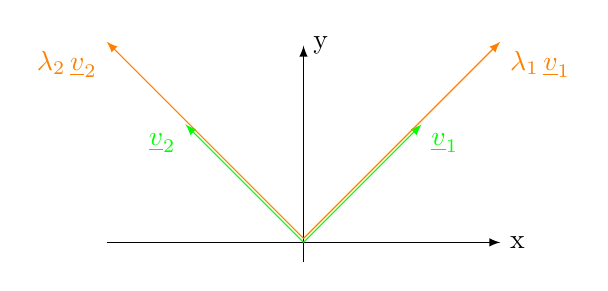
\begin{tikzpicture} [scale =.5]
\draw[-latex] (-5,0) -- (5,0) node [right] {x};
\draw[-latex] (0,-.5) -- (0,5) node[right] {y};

\draw[-latex, green] (0,0) -- (3,3) node[below right] {$\underline{v}_1$};
\draw[-latex, orange] (0,0.1) -- (5,5.1) node[below right] {$\lambda_1\,\underline{v}_1$};

\draw[-latex, green] (0,0) -- (-3,3) node[below left] {$\underline{v}_2$};
\draw[-latex, orange] (0,0.1) -- (-5,5.1) node[below left] {$\lambda_2\,\underline{v}_2$};
\end{tikzpicture}
\end{enumerate}

\paragraph{Def. 14: }
Es sei $\underline{S}$ eine reelle symmetrische Matrix vom Typ $(n,n)$. Die Funktion $y=Q(\underline{x}):=\underline{x}^T\, \underline{S}\, \underline{x}$ ($\underline{x}\in \mathbb{R}^n,\; y \in \mathbb{R}$) heißt \emph{quadratische Form}.
\subparagraph{Diskussion:} 
\begin{enumerate}
\item Im Falle $n=2$ stellt $Q(\underline{x})=const)$ (bzw. $Q(\underline{x})+\underline{a}^T\underline{x=const}$) eine Kurve 2. Ordnung dar. Deren Gestalt kann durch die sogennante Hauptachsentransformation ermittelt werden.
\item Ausführliche Schreibweise $\underline{x}=\begin{pmatrix}
x\\
y
\end{pmatrix},\; \underline{S}=\begin{pmatrix}
s_{11} & s_{12}\\
s_{21} & s_{22}
\end{pmatrix}$ (mit $s_{12}=s_{21}$).\\
$\boxed{Q(x,y)=\begin{pmatrix}
x & y
\end{pmatrix} \begin{pmatrix}
s_{11} & s_{12}\\
s_{21} & s_{22}
\end{pmatrix} \begin{pmatrix}
x\\
y
\end{pmatrix}=s_{11}x^2+2s_{12}xy+s_{22}x^2}$
\item Es seien $\lambda_1$ und $\lambda_2$ die EV von $\underline{S}$ und $\underline{v}_1$ bzw. $\underline{v}_2$ orthonormierte EV. Für einen beliebigen Vektor $\underline{x}=\begin{pmatrix}
x\\
y
\end{pmatrix}\in \mathbb{R}^2$ seien $x^*$ und $y^*$ die Koordinaten bzgl. der Basis $\underline{v}_1, \underline{v}_2$:\\
$\boxed{\underline{x}=x^*\underline{v}_1+y^*\underline{v}_2 = (\underline{v}_1 | \underline{v}_2) \begin{pmatrix}
x^*\\
y^*
\end{pmatrix}=\underline{V}\,\underline{x}^*}$\\
Dann gilt:\\
$\boxed{Q(x,y)=\lambda_1x^{*2}+\lambda_2x^{*2}}$ (Darstellung bzgl. der sog. Hauptachsen)\\
Dann: $Q(x,y)=\underline{x}^T\, \underline{S}\, \underline{x}=\left(\underline{V}\, \underline{x}^*\right)^T \, \underline{S} \, \left( \underline{V} \, \underline{x}^*\right)=\underline{x}^{*T} \underbrace{\underline{V}^T\, \underline{S} \, \underline{V}}_{\Lambda}\underline{x}^*=\begin{pmatrix}
x^*&
y^*
\end{pmatrix} \begin{pmatrix}
\lambda_1 & 0 \\
0 & \lambda_2
\end{pmatrix}\begin{pmatrix}
x^*\\
y^*
\end{pmatrix}\\
\Leftrightarrow Q(x,y)= \lambda_1 x^{*2}+\lambda_2y^{*2}$
\end{enumerate}
\subparagraph{Bsp. 20:} \parskp
$Q(x,,y)=13x^2-32xy+37y^2=45$\\
Welche Kurve ist das?
\begin{itemize}
\item Matrix $\underline{S}$ (vgl. Gleichung aus 2.) aus obiger Diskussion):\\
$\underline{S}=\begin{pmatrix}
13 & -16\\
-16 & 37
\end{pmatrix}$
\item charakteristische Gleichung: \\
$det(\underline{S}-\lambda\underline{E})\overset{!}{=}0 \; \Leftrightarrow \; \begin{vmatrix}
13-\lambda & -16\\
-16 & 37-\lambda
\end{vmatrix}=\lambda^2+50\lambda+225\overset{!}{=}0$\\
$\resultul{\lambda_1=5}, \; \resultul{\lambda_2 = 45}$ (Eigenwerte)
\item EV zu $\lambda_1=5$ ($(\underline{S}-\lambda\underline{E})\underline{x}\overset{!}{=}\underline{x}$):
\begin{align*}
8x-16y &= 0\\
-16x+32y&=0
\end{align*}
$\curvearrowright x=2y \curvearrowright\resultul{\begin{pmatrix}
x\\
y
\end{pmatrix}= \begin{pmatrix}
2t\\
t
\end{pmatrix}=t \begin{pmatrix}
2\\
1
\end{pmatrix}} \quad (t \in \mathbb{R}, t\not = 0)$
\item EV zu $\lambda_2=45$:\\
$\resultul{\begin{pmatrix}
x\\
y
\end{pmatrix}=u\cdot \begin{pmatrix}
1\\
-2
\end{pmatrix}}\quad (u \in \mathbb{R}, u\not = 0)$
\item orthonomierte EV:\\
z.B. $\underline{v}_1=\frac{1}{\sqrt{5}}\begin{pmatrix}
2\\
1
\end{pmatrix}, \; \underline{v}_2=\frac{1}{\sqrt{5}}\begin{pmatrix}
1\\
-2
\end{pmatrix}$ (Rechtssystem!)
\end{itemize}
Mit Gleichung aus 3.) aus obiger Diskussion:\\
$Q(x,y)=\lambda_1x^{*2}+\lambda_2 x^{*2}=5x^{*2}+45y^{*2}=45$\\
$\Leftrightarrow \boxed{\frac{x^{*2}}{9}+\frac{y^{*2}}{1}=1}$ (Ellipse mit Halbachsen $a=3, \; b=1$)